\newchapter{Einleitung}
\label{kap:1}


Partielle Differentialgleichungen sind in vielen Bereichen der Natur- und Ingenieurswissenschaften wiederzufinden. Da die exakte Lösung nicht immer existiert bzw. die Bestimmung solch einer Lösung beliebig kompliziert werden kann, haben numerische Löser für partielle Differnetialgleichungen in den letzen Jahrzehnten mit der Weiterentwicklung des Computers immer mehr an Bedeutung gewonnen. Die Lösung kann daher z.B. mittels \idx{Galerkin-Verfahren} (bzw. Finiter-Elemente-Methode\index{Finite-Elemente-Methode}) ermittelt werden. Hierbei wird die eigentliche Differentialgleichung nur noch approximativ auf einem Gitter gelöst, wobei wir durch Verfeinerung des Gitters die Genauigkeit der Lösung erhöhen, was allerdings auch zu höherem Rechenaufwand führt. Daher ist es sinnvoll die Verfeinerung des Gitters gerade so zu steuern, dass möglichst wenig, aber für eine hinrechend genaue Lösung noch genügend Elemente verfeinert werden. Diese Verfahren werden als \textit{\idx{adaptive Verfeinerungsstategie}n} bezeichnet und sind im Allgemeinen von der Form:
\[
	\text{solve}\ \ \ra \ \ \text{estimate}\ \ \ra\ \ \text{mark}\ \ \ra\  \ \text{refine} \, .
\]
Da die exakte Lösung in den meisten Fällen nicht bekannt ist, ist der Schritt "`estimate"' von entscheidender Bedeutung. Hierbei wird der Fehler zur exakten Lösung auf dem nächsten Gitter mittels eines a posteriori Fehlerschätzer bzgl. des aktuellen Gitters abgeschätzt, was Zuverlässigkeit und Effizienz des Schätzers voraussetzt, d.h. durch Verringerung des Fehlerschätzers wird auch der exakte Fehler kleiner. Im Schritt "`mark"' werden dann dann genau die Elemente ausgewählt, die an dem gewählten Schätzer einen hohen lokalen Anteil haben.

Diese Verfeinerungsstrategien wollen wir in dieser Arbeit zunächst für einen hierarchischen Fehlerschätzer auf einem Hindernisproblem untersuchen. Solche Schätzer basieren auf einer Hierarchie von Ansatzräumen, d.h. man untersucht das gegebene Problem in einem "`besseren"' Finite-Element-Raum und schätzt damit den Fehler bzgl. der "`schlechteren"' \index{Galerkin-Approximation}Galerkin-Appro-ximation ab. Ein Modellproblem eines Hindernisproblems stellt z.B. eine bei Null eingespannte Membran dar, die mit einer Last $f$ vertikal belastet und deren Auslenkung $u: \Omega \ra \R$ durch ein Hindernis $\psi$ behindert wird. Da die in der Membran gespeicherte Energie minimal ist, kann man die Auslenkung dieser durch ein Optimierungsproblem von der Form
\begin{align}\label{eq:1.1}
	u = \arg\min_{v \in K} J(v) = \frac 12 \int_{\Omega} \nabla v \nabla v \, dx - \int_\Omega f v \, dx
\end{align}
modellieren, wobei $K$ die Menge der Auslenkungen $u$ ist, die oberhalb des Hindernisses $\psi$ liegen, d.h. $u\ge \psi$ erfüllen.  In Abbildung \ref{abb:1.1} sind im Vergleich die Auslenkungen einer auf einem Kreisgebiet belasteten Membran ohne und mit (ebenem) Hindernis dargestellt. Für das Problem \eqref{eq:1.1} werden wir in Kapitel \ref{kap:4.1} einen wie oben beschriebenen hierarchischen a posteriori Fehlerschätzer herleiten. Das Hauptresultat befindet sich in Lemma \ref{lem:4.21}, woraus sich das Theorem \ref{theorem:4.22}, welches  die Verwendung des Schätzers ermöglicht, leicht folgern lässt.

\begin{figure}[h]
\begin{center}
\subfigure[ohne Hindernis]{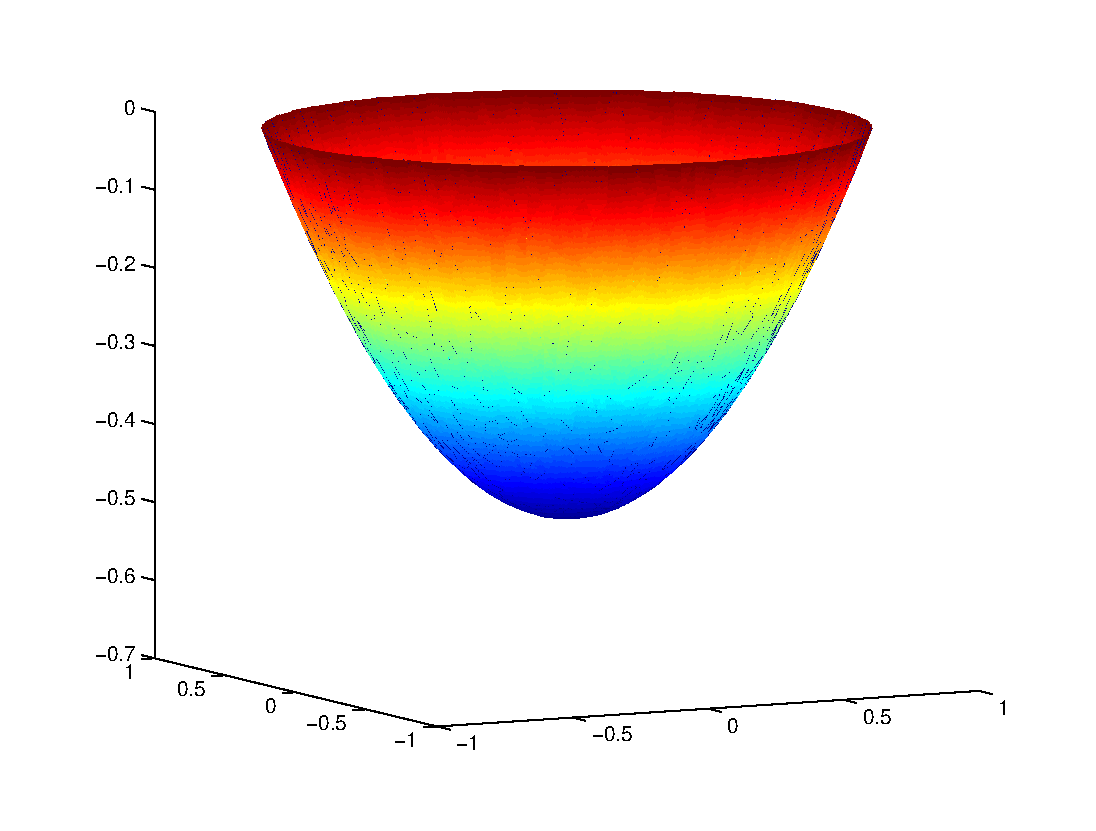
\includegraphics[width=6.25cm]{Abbildungen/bsp_ohne_hindernis.eps}}
\hfill
\subfigure[mit Hindernis: Ebene $z=-0,28$]{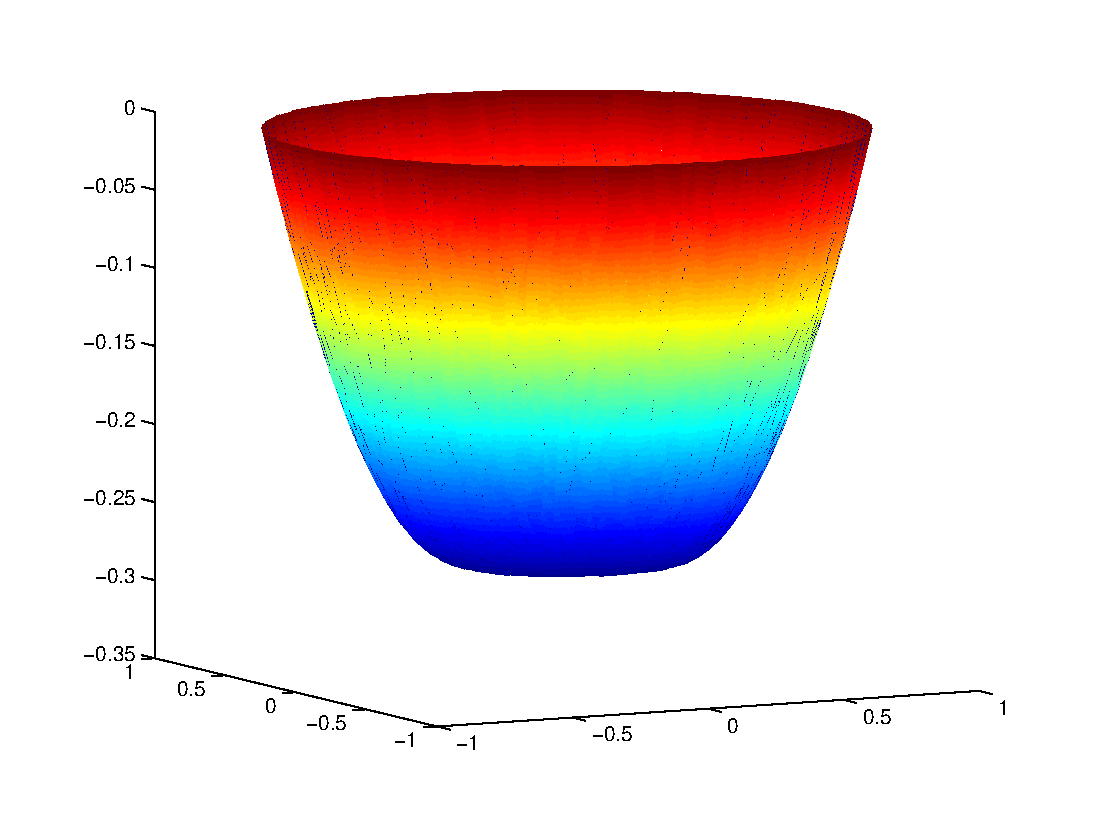
\includegraphics[width=6.25cm]{Abbildungen/bsp_mit_hindernis.eps}}
\end{center}
\caption{Auslenkung einer eingespannten Membran unter Einwirkung einer vertikalen Lastfunktion $f$\label{abb:1.1}}
\end{figure}


Nachdem wir in Kapitel \ref{kap:4} einen hierarchischen a posteriori Fehlerschätzer für das Modellproblem \eqref{eq:1.1} untersucht haben, wollen wir diesen auf Kontaktprobleme übertragen. Kontaktprobleme sind Probleme aus der Strukturmechanik und stellen eine Anwendung von partiellen Differentialgleichungen unter Nebenbedingung (nämlich der Kontaktbedingung) dar. Wir werden uns in dieser Arbeit mit einem vereinfachten Kontaktproblem, dem \textit{\idx{Signorini-Kontakt}problem} beschäftigen, d.h. es gibt keine Reibkräfte auf der Kontaktfläche. Außerdem werden wir von einen linear-elastischen Fall ausgehen. Die Lösung eines Kontaktproblems kann wie oben eindeutig (vgl. Kapitel \ref{kap:3.2}) durch die Minimierung des Energiefunktionals
\begin{align}\label{eq:1.2}
	\mcal J (\bs v) = \frac 12 \int_\Omega \bs \sigma (\bs v):\bs \eps(\bs v) \, d\Omega - \int_\Omega \bs b\cdot \bs v \, d\Omega - \int_{\Gamma} \bs t\cdot \bs v \, d\Gamma 
\end{align}
über $\mscr K$ berechnet werden, wobei die Menge $\mscr K$ diejenigen Verschiebungsfelder $\bs v$ enthält, die die Kontaktbedingung $\bs v \cdot\bs n - g \le 0$ erfüllen. In Kapitel \ref{kap:4.4} werden dann die Übertragungen der Konzepte des Fehlerschätzers für Problem \eqref{eq:1.1} beschrieben.

Zunächst werden wir jedoch in Kapitel \ref{kap:3} zeigen, dass die beiden Probleme \eqref{eq:1.1} und \eqref{eq:1.2} grundlegend auf dieselben Variationsungleichungen führen und die Existenz einer eindeutigen Lösung für diese, und damit auch für die jeweiligen Probleme, zeigen.


Die Lösungsverfahren für die adaptive Verfeinerung der Hindernis- bzw. Kontaktproblemen werden in Matlab implementiert und die wichtigsten Schritte hierfür in Kapitel \ref{kap:5} beschrieben. Der Quellcode ist im Detail im Anhang \ref{anhang:D} einzusehen.

In Kapitel \ref{kap:6} werden wir abschließend mittels der Implementierung die Theorie aus Kapitel \ref{kap:4} anhand mehrerer Beispiele untersuchen.

%
%\begin{itemize}
%\item Thema (worum geht es?) $\ra$ Fehlerabschätzung $\ra$ analytische Lösung oftmals nicht bekannt und damit Fehlerschätzer interessant
%\item[$\ra$] in FEM soll Lösung genauer mit weniger Rechenzeit sein, daraus folgt Anwendung adaptiver Verfahren mit verschiedenen Fehlerschätzern
%\item Lücke zum neuen (Kontaktproblematik) füllen in dieser Arbeit
%\item[$\ra$] Übertragung unseres Fehlerschätzers auf Kontaktprobleme, wie und warum?! $\ra$ möglicher Grund: Hindernisprobleme beinhalten Kontaktbereiche (später für Kapitel 4 interessant)
%\item[wichtig:] Vorgehen einer adaptiven Verfeinerungsstrategie mit "`solve $\ra$ estimate $\ra$ ...."' umschreiben
%\item Struktur der Arbeit
%\item
%\item partielle Differentialgleichungen kommen in vielen Bereichen der Natur- und Ingenieurwissenschaften vor $\Ra$ da die Lösung nicht immer exakt möglich bzw. auch sehr komplex sein kann, approximierte Löser interessant $\Ra$ FEM $\Ra$ Verfeinerung des Gitters (Erhöhung des Freiheitsgrades) bringt genauere Lösung, aber auch mehr Rechenaufwand $\Ra$ so wenig wie möglich verfeinern, d.h. nach Möglichkeit in den Bereichen, in denen der Fehler zur exakten Lösung besondern groß ist $\Ra$ adaptive Verfeinerungsstrategie, allgemein von der Form:
%\[
%	\text{solve}\ \ \ra \ \ \text{estimate}\ \ \ra\ \ \text{mark}\ \ \ra\  \ \text{refine}
%\]
%\item da die exakte Lösung in den meisten Fällen nicht bekannt ist, ist der Schritt 2 entscheidend. die Abschätzung erfolgt mittels eines a posteriori Fehlerschätzers, der den Fehler im nächsten Schritt mit dem aktuellen vergleicht
%\item dies soll Mittelpunkt dieser Arbeit sein.
%\item häufig werden PDE allerdings mit Nebenbedingungen betrachtet, was mittels FEM nicht mehr auf ein LGS führt. 
%\item ein modellproblem hierfür ist das hindernisproblem.
%\item anhand dieses wollen wir einen a posteriori Fehlerschätzer herleiten und dessen Effektivität und Zuverlässigkeit auch an numerischen Beispielen validieren
%\item Kontaktprobleme stellen eine  Anwendung einer PDE unter Nebenbedingung dar. $\Ra$ wir wollen daher in dieser Arbeit auch diese mittels Lösung der FEM untersuchen und den hergeleiteten Fehlerschätzer hierauf übertragen.
%\item Implementiert werden die Lösungsverfahren jeweils in Matlab.
%\item in Kapitel 2 werden wir zunächst grundlegendes einführen; Kapitel 3 enthält die Theorie zur exakten und numerischen Lösbarkeit der Probleme mit a priori Fehlerschätzungen; Kapitel 4 ist das zentrale Kapitel er Arbeit und leitet den betrachteten Fehlerschätzer her mit Übertragung auf Kontakt; Kapitel 5 soll die wichtigsten Ideen der Implementierung in Matlab erläutern; Kapitel 6 ist die numerische Validierung
%\end{itemize}
%
%
%



\newpage

%%% Local Variables: 
%%% mode: latex
%%% TeX-master: "Skript"
%%% End: 
